%%%%%%%%%%%%%%%%%%%%%%%%%%%%%%%%%%%%%%%%%%%%%%%%%%%%%%%%%%%%%%%%%%%%%%%%
\chapter{Supporting {\gpu}s}
%%%%%%%%%%%%%%%%%%%%%%%%%%%%%%%%%%%%%%%%%%%%%%%%%%%%%%%%%%%%%%%%%%%%%%%%

MacSim can model {\gpu}s similar to NVIDIA's Tesla~\cite{lin:nic08} and
Fermi~\cite{fermi} architectures.  In these architectures the {\gpu} consists of a
scalable number of {\em Streaming Multiprocessors} (SMs), each containing
several {\em Scalar Processors} (SP) and {\em Special Function Units} (SFUs), a
multi-threaded instruction fetch and issue unit, a read-only constant cache, and
a read/write scratch pad memory called Shared Memory.  In \SIM, SMs are modeled
as cores and SPs as just one of the functional units. 


		\begin{figure}[htb]
		\centering
		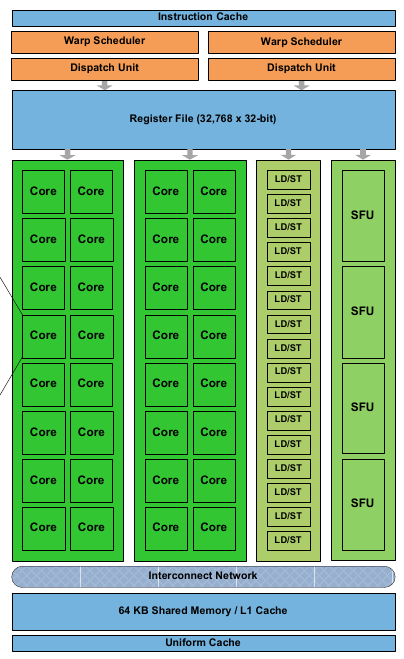
\includegraphics[scale=0.5]{figs/fermi_arch.png}
		\caption{An overview of the Fermi {\gpu} architecture}
		\label{fig:g80}
		\end{figure}

The behavior of certain components is different when simulating {\gpu}s, these
differences are described briefly below.

%%%%%%%%%%%%%%%%%%%%%%%%%%%%%%%%%%%%%%%%%%%%%%%%%%%%%%%%%%%%%%%%%%%%%%%%
\section{Traces}
\label{sec:ptx_traces}
%%%%%%%%%%%%%%%%%%%%%%%%%%%%%%%%%%%%%%%%%%%%%%%%%%%%%%%%%%%%%%%%%%%%%%%%

In NVIDIA {\gpu}s threads are executed in batches of 32 threads called
\textit{warps}. For simulating execution at warp granularity, for {\gpu}
applications, we generate traces at warp granularity. This means there
is one trace file per warp and each instruction in a trace file represents an
instruction executed by a warp. The instruction in the trace file encodes which
threads in the warp were active during the execution of the instruction. For
divergent branches, all instructions from one path are written to the trace
file first and only then instructions from the other path are written to the
trace file. For memory instructions, multiple instructions are written to the
trace file since each thread in a warp can access different addresses. Handling
of memory instructions inside the simulator is explained below.


%%%%%%%%%%%%%%%%%%%%%%%%%%%%%%%%%%%%%%%%%%%%%%%%%%%%%%%%%%%%%%%%%%%%%%%%
\section{Process Manager}
%%%%%%%%%%%%%%%%%%%%%%%%%%%%%%%%%%%%%%%%%%%%%%%%%%%%%%%%%%%%%%%%%%%%%%%%

The Process Manager (explained in Chapter~\ref{sec:process_manager})
does assignment of threads to cores (SMs) at block granularity - all
warps in the same thread block are assigned to the same core. The
number of blocks that can be assigned to each core is determined from
the resource requirement of each block and the {\gpu} architecture being
simulated.  This number is calculated at the time of trace generation
for compute devices of capability 2.0 and is included in the trace
files. This can also be specified by setting the knob
\Verb+max_block_per_core_super+.  For each block, the Process Manager
tracks the number of completed warps and when all warps in a block
have completed, the Process Manager retires the block and assigns a
new block to the core. The policy for assigning blocks to cores can be
different. Blocks could either be assigned statically to cores, or they
can be assigned to the first core that can accommodate the new block.

\ignore
		{\todo[inline]{support ..\_per\_core\_super per application}}

%%%%%%%%%%%%%%%%%%%%%%%%%%%%%%%%%%%%%%%%%%%%%%%%%%%%%%%%%%%%%%%%%%%%%%%%
\section{Memory Hierarchy}
%%%%%%%%%%%%%%%%%%%%%%%%%%%%%%%%%%%%%%%%%%%%%%%%%%%%%%%%%%%%%%%%%%%%%%%%

The following new components are added to the memory hierarchy for  - Shared Memory,
    Const Cache, Texture Cache.

%%%%%%%%%%%%%%%%%%%%%%%%%%%%%%%%%%%%%%%%%%%%%%%%%%%%%%%%%%%%%%%%%%%%%%%%
\section{Instruction Scheduler}
%%%%%%%%%%%%%%%%%%%%%%%%%%%%%%%%%%%%%%%%%%%%%%%%%%%%%%%%%%%%%%%%%%%%%%%%

A {\gpu}-specific (or a multithreaded architecture specific) instruction
scheduler is necessary, since neither single-threaded in-order nor
single-threaded out-of-order schedulers match the requirement of a {\gpu}
scheduler. A {\gpu} scheduler must be able to schedule instructions from
different warps while scheduling instructions from the same warp
in-order. A {\gpu}-specific scheduler is implemented in
\Verb+schedule_smc.cc+, this scheduler chooses instructions from
different warps. 

\ignore{\todo{round-robin order - not true!}}.

%%%%%%%%%%%%%%%%%%%%%%%%%%%%%%%%%%%%%%%%%%%%%%%%%%%%%%%%%%%%%%%%%%%%%%%%
\section{Simulating Memory Instructions}
%%%%%%%%%%%%%%%%%%%%%%%%%%%%%%%%%%%%%%%%%%%%%%%%%%%%%%%%%%%%%%%%%%%%%%%%

Due to the execution of threads at warp granularity, the execution of a memory
instruction generates multiple addresses, one from each thread. In the trace
file all the memory accesses are included as individual trace instructions, but
the accesses are marked as generated from the same memory instruction. During
simulation when it is detected that a sequence of memory accesses are from the
same memory instruction, the trace is read ahead until the end of the sequence
and the individual memory accesses are attached to a main uop as child uops. It
is the main uop that flows through the pipeline stages until execution. In the
execution stage it is detected that the main uop has several child uops and the
child uops that are issued to the memory hierarchy. When all the child uops
have completed, the main uop is ready for retirement.

\ignore
	  {
	  \missingfigure{better to add diagram from slide}
	  }

\ignore 
		{
		\subsection{Changes to support {\gpu}}
		\subsubsection{Front-end changes}
		The following components are modified to support {\gpu}s. 
		\begin{enumerate}
		\item Handling divergent branch
		\item Fetch scheduling (when to block a thread)
		\end{enumerate}
		\subsubsection{Scheduler}
		Different scheduling policy can be implemented. The default is the round-robin policy. 

		\subsubsection{Process Manager}

		\begin{enumerate}
		\item Block Dispatch: Threads are dispatched as a block granularity. 
		The simulator waits until all threads within a block are finished 
		before it dispatches another block. 
		\item Occupancy: When a trace is generated from Ocelot, it also emits the number of required 
		physical registers and memory usages. So the simulator uses that information to decide 
		how many blocks can be allocated for each core. This value can be overwritten by a KNOB as well. 
		\end{enumerate}

		\subsubsection{Execution Stage}
		Since one warp is treated as a functional unit, execution stage itself does not require too much change. Major changes are in handling uncoalesced memory  requests. 

		\subsubsection{Memory system}
		The simulator includes read-only cache, texture cache and constant cache to model {\gpu}s. 
		}

\ignore
		{
		Executing a warp instruction applies the instruction to 32 threads, similar to
		executing a SIMD instruction like an SSE instruction~\cite{sse} in X86.
		However, unlike SIMD instructions, the concept of warp is not exposed to the
		programmers, rather programmers write a program for one thread, and then
		specify the number of parallel threads in a block, and the number of blocks
		in a kernel grid. The Tesla architecture forms a warp using a batch of 32
		threads~\cite{cuda:course, sc2008_cuda} and in the rest of the paper we also
		use a warp as a batch of 32 threads.\ignore{\footnote{The CUDA
		manual~\cite{cuda_manual} describes a half warp (16 threads) as a minimum
		unit of execution. However, to simplify the model, we use only warp as a
		minimum unit of execution.}}

		All the threads in one block are executed on one SM together. One SM
		can also have multiple concurrently running blocks. The number of
		blocks that are running on one SM is determined by the resource
		requirements of each block such as the number of registers and shared
		memory usage. The blocks that are running on one SM at a given time
		are called {\em active blocks} in this paper. Since one block
		typically has several warps (the number of warps is the same as the
		number of threads in a block divided by 32), the total number of
		active warps per SM is equal to the number of warps per block times
		the number of active blocks.

		The shared memory is implemented within each SM multiprocessor as an
		SRAM and the global memory is part of the offchip DRAM. The shared
		memory has very low access latency (almost the same as that of
		register) and high bandwidth. However, since a warp of 32 threads
		access the shared memory together, when there is a bank conflict
		within a warp, accessing the shared memory takes multiple cycles.
		}


% LocalWords:  {\gpu} NVIDIA SMs SFUs multithreaded SPs {\gpu}s uncoalesced SIMD CUDA
% LocalWords:  SRAM offchip
